% Copyright 2024 Kieran W Harvie. All rights reserved.

\section{Sedrakyan Ellipse}
Sedrakyan's inequality states that for positive reals $a$ and $b$ we have:
\[\frac{(x+y)^2}{a+b} \leq \frac{x^2}{a}+\frac{y^2}{b}\]
With equality iff there exists $k$ such that:
\[x=ka,\,y=kb\]
Simple manipulation gives:
\[2xy \leq rx^2+r^{-1}y^2\quad r = \frac{a}{b}\]
With equality iff:
\[y=rx\]
Both sides have a direct geometric interpretation as an ellipse and hyperbola,
by setting both sides equal a constant (WLOG $1$).
And the ellipse is contained within the hyperbola:
\begin{center}
\begin{tikzpicture}[every node/.style={black}]
	\draw plot[variable=\x, samples=200,domain=0.25:2.5] ({\x},{1/(2*\x)});
	\draw plot[variable=\x, samples=200,domain=-0.25:-2.5] ({\x},{1/(2*\x)});
	\draw[red] (0,0) ellipse (1.5 and 0.666666);
\end{tikzpicture}
\end{center}
I'm not the most brushed up on algebraic varieties, 
so perhaps there is more direct proof,
but I know it doesn't follow from:
\[f(x,y)\leq g(x,y)\]
That $f(x,y)=1$ is contained in $g(x,y)=1$, 
or vise versa.
This can be seen by considering circles and noting that we can easily change the radii with:
\[h(x,y)=f(x,y)\pm r\]

But the inequality does also have an equality condition that $y=rx$,
these intersect with the hyperbola at $(\pm r,\pm\frac{1}{2r})$.
These intersect occur once at each branch of the hyperbola,
and the hyperbola's branches divides the plane into three disconnected spaces.
Hence the ellipse in wholly in the central space.
Because for the ellipse to cross a second space requires crossing the same branch at least twice.
\\

Again there's likely a more rigours and direct proof then the above one,
but I'm not brushed up.
If I had to provide a more rigorous argument I would calculate the tangents for the figures at $(\pm r,\pm\frac{1}{2r})$.
\\

Another interesting observation is the ellipses have area $1$ and,
if you reflect he hyperbola,
intersects then four times:
\begin{center}
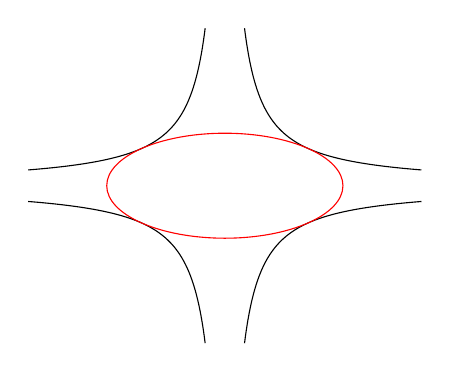
\begin{tikzpicture}[every node/.style={black}]
	\draw plot[variable=\x, samples=200,domain=0.25:2.5] ({\x},{1/(2*\x)});
	\draw plot[variable=\x, samples=200,domain=-0.25:-2.5] ({\x},{1/(2*\x)});
	\draw plot[variable=\x, samples=200,domain=0.25:2.5] ({\x},{-1/(2*\x)});
	\draw plot[variable=\x, samples=200,domain=-0.25:-2.5] ({\x},{-1/(2*\x)});
	\draw[red] (0,0) ellipse (1.5 and 0.666666);
\end{tikzpicture}
\end{center}
There seems to be enough symmetry here to say that the largest area an ellipse can obtain in the area between hyperbolas is $1$.
Especially since how well hyperbolas act when scaling the axes while maintaining area.
